\documentclass[../diplomski_rad.tex]{subfiles}

\begin{document}

\sloppy

\justifying

Laboratorijska mjerenja provedena su u SleepdB laboratoriju (KITE Toronto Rehabilitation Institute, 
University Health Network, Toronto, Kanada). 
Istraživanje je odobrio Odbor za etičko istraživanje (University Health Network Research Ethics Board) (REB 18 5090). 
Svi ispitanici dali su pisani pristanak prije sudjelovanja u istraživanju. 
U istraživanju je sudjelovalo šest ispitanika čiji demografski podaci su prikazani u tablici \ref{tab:opci_podaci}, 
a mjerenja su provedena korištenjem razvijenog mjernog sustava (Slika X) 
i ranije opisanog SFB7 ImpediMed sustava \cite{sfb7}, koji se smatra zlatnim standardom. 
Također, uspoređeni su rezultati mjerenja dobiveni gel elektrodama s onima dobivenim tekstilnim elektrodama. 
Mjerni sustav je prikazan slikom X, gdje su vidljivi svi prethodno opisani dijelovi mjernog sustava.

\begin{table}[H]
    \centering
    \begin{tblr}{
        width=1\linewidth,
        cells={valign=m,halign=c},
        row{1}={bg=lightgray,font=\bfseries,rowsep=8pt},
        hlines,
        vlines
    }
        \hline
        Broj ispitanika & Dob (godina) & Visina (cm) & Težina (kg) & BMI \\ [0.5ex] 
        \hline\hline
        6 & 26±5.44  & 174.16±12.09 & 74±15.61 & 24.28±3.65 \\
        \hline
    \end{tblr}
    \caption{\label{tab:opci_podaci}Demografski podaci}
    \end{table}
    
Zbog svoje praktičnosti, udobnosti i kompatibilnosti, tekstilne elektrode sve više se integriraju u pametna nosiva 
rješenja kao preferirani izbor za praćenje zdravstvenih parametara, uključujući distribuciju tekućine. 
Tekstilne elektrode korištene u ovom radu nude neinvazivno i nosivo rješenje, omogućujući dugotrajno praćenje tekućine, 
posebno kod osoba sa srčanim zatajenjem \cite{McDonald2010},\cite{Gudmundsson2016}. 
Korištene su tekstilne elektrode razvijene unutar SleepdB istraživačke grupe \cite{Piper2023}. 
Tekstilne elektrode se temelje na vodljivom srebrenom materijalu, prikazane na slici \ref{slk:tekstilne_elektrode}, 
a koje su posebno dizajnirane za praćenje tekućine.

\begin{figure}[htb]
    \centering
    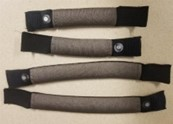
\includegraphics[width=0.45\textwidth]{Figures/tekstilne_elektrode.jpg} 
    \caption{Trake s tekstilnim elektrodama na bazi srebra koje pokrivaju cijeli opseg za praćenje tekućine \cite{Bandur2023}}
    \label{slk:tekstilne_elektrode}
\end{figure}

\section{Protokol mjerenja}

Razvijeni nosivi bežični sustav mjeri bioimpedanciju te BLE komunikacijskim protokolom šalje na udaljenu desktop aplikaciju. 
Aplikacija obavlja daljnje izračune volumena tekućine u tijelu i nogama. 
Korištena su dobivena mjerenja impedancije tijela za izračun volumena tekućine u tijelu koristeći MF BIA funkcije opisane u \cite{Sanchez2013}. 
Za izračun volumena tekućine u nozi, korištene su funkcije opisane u \cite{Delano2022}.

Za validaciju ispravnosti rada mjernog sustava provedena je vježba plantarne fleksija, 
prikazano na slici \ref{slk:plantarna_fleksija}, gdje je pozicija A neutralni položaj, 
gdje je stopalo ravno na tlu, a pozicija B je plantarna fleksija, gdje je stopalo usmjereno prema dolje. 
Plantarna fleksija u ovom radu koristi se za validaciju promjene tekućine u nogama jer aktivira 
mišiće gastrocnemius i soleus, što može potaknuti cirkulaciju krvi i limfne tekućine. 
Tijekom ove vježbe, pritisak na poplitealnu venu može poslužiti kao indikacija promjena u volumenu tekućine. 
Stoga, praćenje plantarne fleksije može pružiti vrijedne podatke o dinamici tekućine u donjim ekstremitetima, 
što je posebno korisno za pacijente sa srčanim zatajenjem ili drugim sličnim stanjima \cite{AVILADEOLIVEIRA2022102625}. 

\begin{figure}[htb]
    \centering
    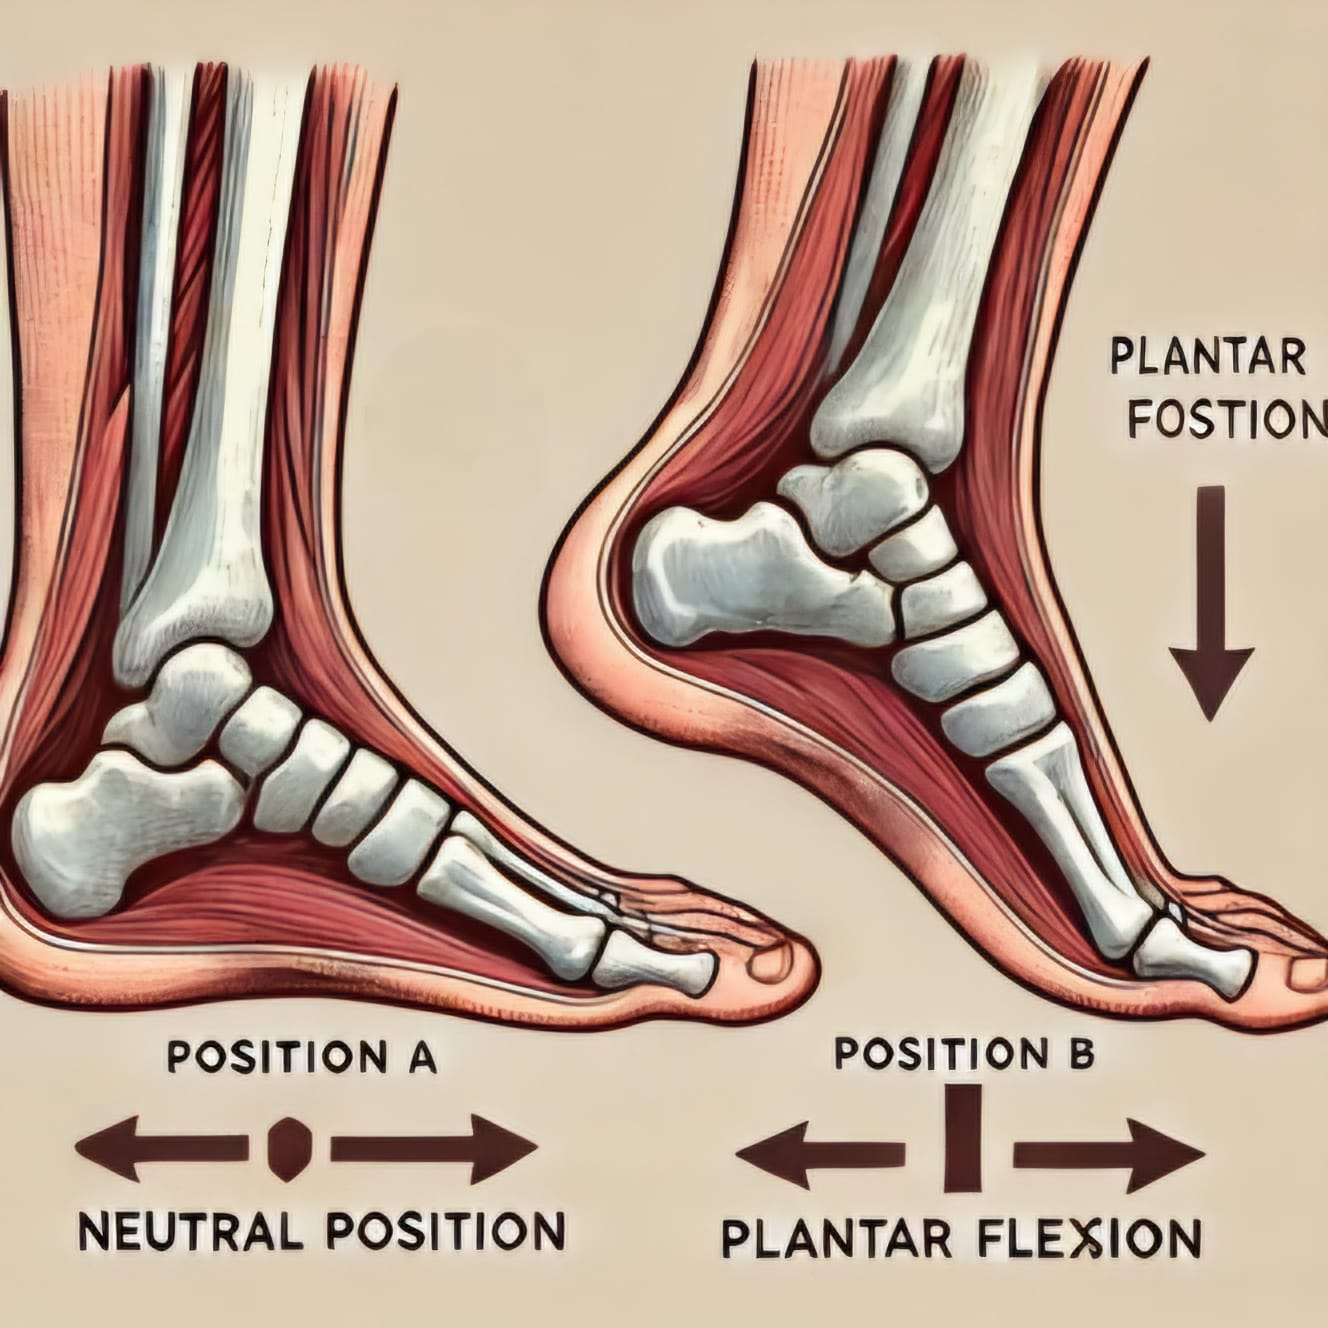
\includegraphics[width=0.45\textwidth]{Figures/plantarna_fleksija.jpg} 
    \caption{Ilustracija prikazuje neutralnu poziciju (A) i plantarnu fleksiju (B) stopala \newline (generirano pomoću DALL-E alata iz OpenAI)
    }
    \label{slk:plantarna_fleksija}
\end{figure}

U radu je provedeno kontinuirano ponavljanje pokreta plantarne fleksije pet minuta prema slici A, 
kako bi se odredilo učinkovita procjena promjene volumena tekućine u nogama.

- slika protokola

Hipoteza je da bi kontinuirano ponavljanje pokreta tijekom 5 minuta bilo učinkovitije u promjeni volumena 
tekućine u nogama u usporedbi s povremenim ponavljanjem pokreta s pauzama. 
Kontinuirana kontrakcija mišića osigurava stalni pritisak na poplitealnu venu, 
što bi trebalo rezultirati bržim smanjenjem tekućine u nogama zbog povećanog venskog povratka.

Tijekom mjerenja, na desnu potkoljenicu ispitanika postavljene su gel elektrode na istoj razini kao i 
tekstilne elektrode kako bi se osiguralo prikupljanje podataka s istog dijela tijela. 
Početno mjerenje cjelokupnog sastava tijela obavljeno je pomoću ImpediMed SFB7 dok je ispitanik bio u stojećem položaju. 
Mjerenje je dobiveno postavljanjem elektroda na zapešće desne ruke i gležanj desne noge. 
Za analizu impedancije noge, elektrode su bile postavljene na koljeno i gležanj desne noge.

Gel i tekstilne elektrode postavljene su na istoj visini na desnoj nozi sudionika, osiguravajući da se 
vodljivi tekstil ne preklapa s gel elektrodom \cite{Piper2023}. 
Elektrode su postavljene s minimalnim razmakom od 2 cm između parova. 
Također, za svakog ispitanika izmjeren je opseg oko koljena, gležnja i najšireg dijela lista, 
kao i udaljenost između dviju senzorskih (V+ i V-) elektroda.

\section{Analiza podataka}

Softver BioIMP, ImpediMed Inc., korišten je za generiranje automatskih granica iz sirovih 
vrijednosti otpora i reaktancije izmjerenih uređajem SFB7. 
Točke podataka koje su odstupale više od 1\% od izračunate krivulje isključene 
su iz izračuna vrijednosti $R_{0}$ i $R_{\infty}$ \cite{Piper2023}. 
Te vrijednosti uzimaju se kao x-presjeci u Cole-Cole dijagramu (negativna reaktancija vs. otpor) 
i koriste se za izračun volumena tekućine. 
U svakoj iteraciji, procijenjene vrijednosti $R_{0}$ i $R_{\infty}$ dobivene tekstilnim elektrodama uspoređene
su s vrijednostima zlatnog standarda gel elektroda koristeći korelacijsku analizu i korijen 
srednje kvadratne pogreške (RMSE) između dvaju mjerenja \cite{Piper2023}.

Također, prije početka mjernog procesa, izmjereni su određeni segmenti tijela (Tablica \ref{tab:segmenti_tijela}) i 
prikupljeni su demografski podaci ispitanika (Tablica \ref{tab:opci_podaci}), 
koji su korišteni u jednadžbama \cite{Sanchez2013}, \cite{Delano2022} za procjenu volumena tekućine.


\begin{table}[H]
\centering
\begin{tblr}{
    width=1\linewidth,
    cells={valign=m,halign=c},
    row{1}={bg=lightgray,font=\bfseries,rowsep=8pt},
    cell{1}{1} = {c = 3}{halign = c},
    cell{1}{4} = {r = 2}{valign = m},
    hlines,
    vlines
}
    \hline
    Opseg &  &  & Razmak elektroda \\ [0.5ex] 
    \hline
    Gležanj & List & Koljeno &  \\ [0.5ex] 
    \hline\hline
    23.48±1.30 & 36.92±53.46  & 34.92±2.90 & 10.07±3.09  \\
    \hline
\end{tblr}
\caption{\label{tab:segmenti_tijela}Izmjereni segmenti tijela}
\end{table}

\end{document}